\prefacesection{Feasibility}

\section*{Technical Requirements}
There are a number technologies and services that will be required in order to achieve the end goal of this research project. For a better understanding, the requirements are broken into categories that provide the a brief technical background on how they work and what they will be used for. 

\subsection*{Language}
For a data science project, there are many languages that accommodate fast calculation speeds and handling of big data sets. Two of the most prevalent languages for data science Python and R \citep{frossbytes}. Each language has their strengths and weaknesses.
\subsubsection{Python}
Python is highly recommended for data science projects as it is heavily documented, holds a large community and it is considered to easier to learn than R. Python supports many machine learning libraries that are regularly maintained. Furthermore, Python is renowned for is capability of handling big data in contrast to R.
\subsubsection{R}
R is considered to be the most prominent language for data science. Although it is regarded as a strong candidate for this project, the main downfalls it has is its lack of ability to handle large data loads like Python, and because it is looked upon as a harder language to grasp. Some benefits of this language be the computation speed it provides, unlike Python.

\subsection*{Machine Learning Libraries}
Software libraries prove to be very beneficial in implementing machine learning (ML) models as they reduce the complexity and program length \citep{jain_2017}. The most prominent ML libraries used today are Caffe, Scikit Learn and Tensorflow. 
\subsubsection{TensorFlow}
TensorFlow is an open source machine learning library developed by the Google Brain team. It can be run on CPUs, GPUs and mobile platforms. For machine learning algorithms, such as gradient descent, TensorFlow provides automatic differentiation which can prove to be very advantageous in comparison to other ML libraries. It also supports multiple languages such as Python, Java and C++ and Go \citep{jain_2017}. Graph visualisation is also supported. Multi-threading is also achievable with the use of TensorFlow
\subsubsection{Scikit Learn}
Scikit Learn is an open source machine intelligence built on top of other libraries such as Matplotlib, SciPy and NumPy. A good feature that Scikit Learn incorporates is the ability of evaluating, chaining and adjusting model hyper parameters \citep{jain_2017}.
\subsubsection{Caffe}
Caffe is a ML library that focuses on speed and modularity and is mainly utilized for convolutional neural networks and computer vision. Another selling point for Caffe is it's pre-trained models that do not require any coding or training. It supports GPU and CPU computations but a disadvantage of this library is that it is specifically for application implementation, not for research and development \citep{koshy_2017}. 


\subsection*{Web Frameworks}
A web framework will required to run the application on a server, and to aid in building the front end. The framework should be lightweight, fast and easy to implement to reduce time consumption in the development of the project. A number of considerable web frameworks for this project revolve either in Node.JS or Python. 
\subsubsection{Flask}
Flask is a modular Python web framework that known for being very easy to set up. Flask provides the option of have or not have an ORM. It is highly supported and considered to be one of the most popular frameworks for ease of use \citep{slant}. 
A downfall of this framework is its design to not support asynchronous programming.
\subsubsection{Express}
Express is a powerful Node.JS module that provides route building for RESTful API development. Express is seen as a relatively old module therefore it has a strong community backing. It is also considered to be a very straightforward and uncomplicated framework and would be benign to the implementation of the project \citep{slant}.

\subsection*{Training Platform/Setup}
For model training, there are two approaches that can be taken in order to train and improve the accuracy of the model: to train locally on the host machine or to use a cloud platform. The are pros and cons to both approaches. Training locally is the cheaper option, but it requires exceptional computing power in order to train a convolutional neural network due to the large image dataset, which may not be accessible. The through a cloud platform provides dedicated hardware for training and they are highly accessible, they do require payment for anything beyond the basic tier plans. Additionally, a labelled dataset of human emotional expression is required for training.
\subsubsection{Distributed TesnorFlow}
For training locally, TensorFlow provides the mean to create your own cluster of servers in order to divide the work load of your training to implement distributed deep learning \citep{dist}. Each node in the cluster are known as "tasks".  There is a master node that distributes jobs to each task accordingly. A node in the cluster can receive either one or more jobs to do and run that task's hardware.

\begin{figure}[ht]
	\begin{center}
		\advance\leftskip-3cm
		\advance\rightskip-3cm
		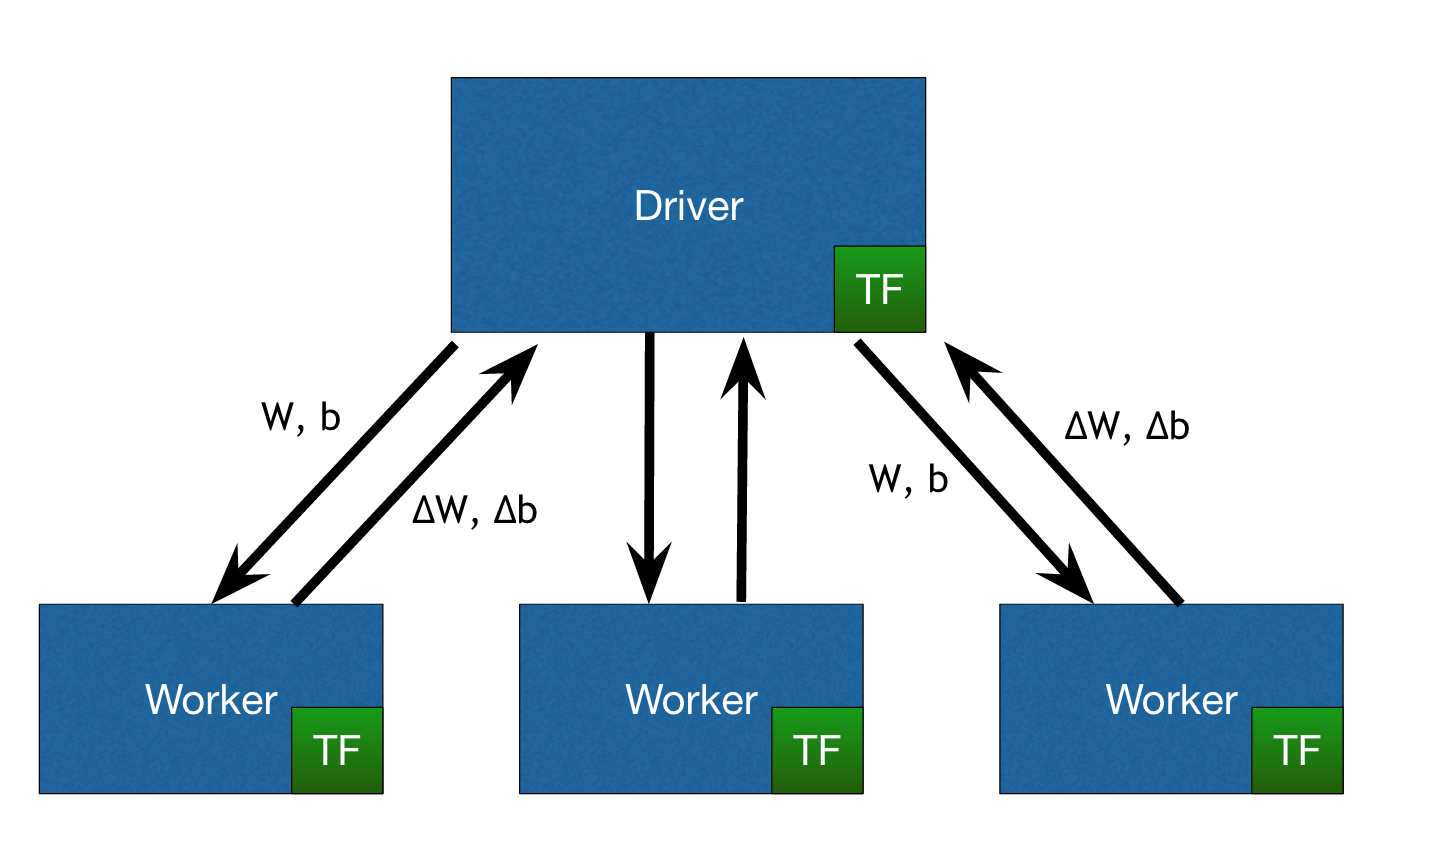
\includegraphics[keepaspectratio=true,scale=0.3]{resources/dist.jpg}
		\label{fig: Distributed TensorFlow},
		\caption{Distributed TensorFlow Topology}
		\label{pop}
	\end{center}
\end{figure}

\subsubsection{TensorPort}
TensorPort is a distributed machine training platform specifically for TensorFlow developed by Good AI Lab. The free tier provides 10GB's of storage, five graphical processing units and twenty central processing units. Additionally, TensorPort allows a number of integrations. Git VCS and TensorBoard (Graph visualisation) is integrated on the online portal. Lastly, it also provides Keras support, should it be needed.




